% Author: Izaak Neutelings (November 2020)
\documentclass[border=3pt,tikz]{standalone}
\usepackage{amsmath} % for \dfrac
\usepackage{physics,siunitx}
\usepackage{tikz,pgfplots}
\usepackage[outline]{contour} % glow around text
\contourlength{1.0pt}
\usetikzlibrary{angles,quotes} % for pic (angle labels)
\usetikzlibrary{arrows.meta}
\usetikzlibrary{decorations.markings}
\tikzset{>=latex} % for LaTeX arrow head
\usepackage{xcolor}

\colorlet{xcol}{blue!60!black}
\colorlet{myred}{red!85!black}
\colorlet{myblue}{blue!80!black}
\colorlet{mycyan}{cyan!80!black}
\colorlet{mygreen}{green!70!black}
\colorlet{myorange}{orange!90!black!80}
\colorlet{mypurple}{red!50!blue!90!black!80}
\colorlet{mydarkred}{myred!80!black}
\colorlet{mydarkblue}{myblue!80!black}
\tikzstyle{xline}=[xcol,thick]
\tikzstyle{Tline}=[line width=0.6]
\tikzstyle{width}=[{Latex[length=5,width=3]}-{Latex[length=5,width=3]},thick]
\def\tick#1#2{\draw[thick] (#1)++(#2:0.12) --++ (#2-180:0.24)}
\def\N{100} % number of samples


\begin{document}


% POLYNOMIAL
% y = (x+1)*(x-1)^2
%   = x^3-x^2-x+1
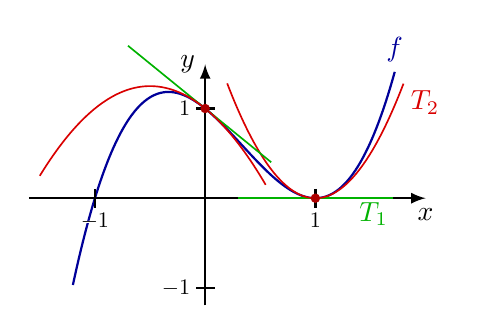
\begin{tikzpicture}
  \message{^^JPolynomial}
  \def\a{(0.5*\xmax)} % root
  \def\A{(0.67*\ymax)} % amplitude
  \def\xmax{2.8}    % max x axis
  \def\ymax{1.7}    % max y axis
  
  % AXIS
  \draw[->,thick] (0,-0.8*\ymax) -- (0,\ymax) node[left] {$y$};
  \draw[->,thick] (-0.8*\xmax,0) -- (\xmax,0) node[below] {$x$};
  
  % PLOT
  \draw[xline,samples=\N,smooth,variable=\x,domain=-0.6*\xmax:0.86*\xmax]
    plot(\x,{\A/\a^3*(\x+\a)*(\x-\a)^2}) node[above] {$f$};
  \draw[Tline,mygreen,samples=\N,smooth,variable=\x,domain=0.3*\a:1.7*\a]
    plot(\x,0) node[below left=-2] {$T_1$};
  \draw[Tline,myred,samples=\N,smooth,variable=\x,domain=0.2*\a:1.8*\a]
    plot(\x,{\A/\a^3*2*\a*(\x-\a)^2}) node[below right=-1] {$T_2$};
  \draw[Tline,mygreen,samples=\N,smooth,variable=\x,domain=-0.7*\a:0.6*\a]
    plot(\x,{\A/\a^3*(\a^3-\a^2*\x)});
  \draw[Tline,myred,samples=\N,smooth,variable=\x,domain=-1.5*\a:0.55*\a]
    plot(\x,{\A/\a^3*(\a^3-\a^2*\x-\a*\x*\x)});
  %\node[xcol,above=2,right=4] at ({720/\om},\A) {$x(t)=A\cos(\omega t)$};
  
  \tick{0,{\A}}{0} node[left=-1,scale=0.8] {$1$};
  \tick{0,{-\A}}{0} node[left=-1,scale=0.8] {$-1$};
  \tick{{\a},0}{90} node[below=-1,scale=0.8] {$1$};
  \tick{{-\a},0}{90} node[below=-1,scale=0.8] {\contour{white}{$-1$}};
  \fill[myred!80!black] (0,{\A}) circle(0.06);
  \fill[myred!80!black] ({\a},0) circle(0.06);
  
\end{tikzpicture}


% COS
\def\A{0.8}    % amplitude
\def\om{(1.4*2*pi/(0.94*\xmax))} % angular frequency in radians
\def\T{(2*pi/\om))} % period
\def\xmax{3.2} % max x axis
\def\ymax{1.2} % max y axis
\begin{tikzpicture}
  \message{^^JCosine}
  \draw[->,thick] (0,-\ymax) -- (0,1.1*\ymax) node[left] {$y$};
  \draw[->,thick] (-\xmax,0) -- (\xmax,0) node[below] {$x$};
  \draw[xline,samples=100+\N,smooth,variable=\x,domain=-0.94*\xmax:0.94*\xmax]
    plot(\x,{\A*cos(\om*180/pi*\x)})
    node[below=0] {$\cos$};
  \draw[Tline,mygreen,samples=\N,smooth,variable=\x,domain={-0.26*\T}:{0.26*\T}]
    plot(\x,\A)
    node[above=0] {$T_0$};
  \draw[Tline,myred,samples=\N,smooth,variable=\x,domain={-0.32*\T}:{0.32*\T}]
    plot(\x,{\A*(1-\om^2/2*(\x)^2)})
    node[below=0] {$T_2$};
  \draw[Tline,myorange,samples=\N,smooth,variable=\x,domain={0.55*\T}:{-0.55*\T}]
    plot(\x,{\A*(1-\om^2/2*(\x)^2+\om^4/24*(\x)^4)})
    node[above] {$T_4$};
  \draw[Tline,mypurple,samples=\N,smooth,variable=\x,domain={0.51*\T}:{-0.51*\T}]
    plot(\x,{\A*(1-\om^2/2*(\x)^2+\om^4/24*(\x)^4-\om^6/720*(\x)^6)})
    node[below] {$T_6$};
  \draw[Tline,mycyan,samples=\N,smooth,variable=\x,domain={-0.73*\T}:{0.73*\T}]
    plot(\x,{\A*(1-\om^2/2*(\x)^2+\om^4/24*(\x)^4-\om^6/720*(\x)^6+(\om/3.76435*\x)^8)})
    node[above] {$T_8$}; %40320
  \fill[myred!80!black] (0,\A) circle(0.06);
  \tick{{\T},0}{90} node[below=0,scale=0.8] {$T$};
  \tick{{-\T},0}{90} node[below=0,scale=0.8] {$-T$};
\end{tikzpicture}


% SIN
\begin{tikzpicture}
  \message{^^JSine}
  \draw[->,thick] (0,-\ymax) -- (0,1.1*\ymax) node[left] {$y$};
  \draw[->,thick] (-\xmax,0) -- (\xmax,0) node[below] {$x$};
  \draw[xline,samples=100+\N,smooth,variable=\x,domain=-0.94*\xmax:0.94*\xmax]
    plot(\x,{\A*sin(\om*180/pi*\x)})
    node[right=0] {$\sin$};
  \draw[Tline,mygreen,samples=\N,smooth,variable=\x,domain={-0.22*\T}:{0.22*\T}]
    plot(\x,{\A*\om*\x})
    node[right=0] {$T_1$};
  \draw[Tline,myred,samples=\N,smooth,variable=\x,domain={-0.43*\T}:{0.43*\T}]
    plot(\x,{\A*(\om*\x-\om^3/6*(\x)^3)})
    node[below=0] {$T_3$};
  \draw[Tline,myorange,samples=\N,smooth,variable=\x,domain={0.55*\T}:{-0.55*\T}]
    plot(\x,{\A*(\om*\x-\om^3/6*(\x)^3+\om^5/120*(\x)^5)})
    node[below left=-2] {$T_5$};
  \draw[Tline,mypurple,samples=\N,smooth,variable=\x,domain={0.61*\T}:{-0.61*\T}]
    plot(\x,{\A*(\om*\x-\om^3/6*(\x)^3+\om^5/120*(\x)^5-(\om/3.38*\x)^7)})
    node[above] {$T_7$};
  \draw[Tline,mycyan,samples=\N,smooth,variable=\x,domain={-0.82*\T}:{0.82*\T}]
    plot(\x,{\A*(\om*\x-\om^3/6*(\x)^3+\om^5/120*(\x)^5-(\om/3.38*\x)^7+(\om/4.1472*\x)^9)})
    node[above] {$T_9$};
  \fill[myred!80!black] (0,0) circle(0.06);
  \tick{{\T},0}{90} node[right=3,below=0,scale=0.8] {$T$};
  \tick{{-\T},0}{90} node[right=2,below=0,scale=0.8] {$-T$};
\end{tikzpicture}


% COS - difference
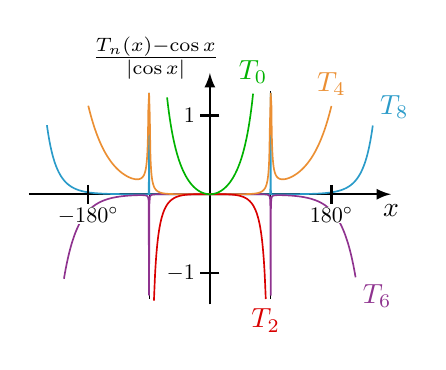
\begin{tikzpicture}
  \message{^^JCosine difference}
  \def\A{1.0}    % amplitude
  \def\xmax{2.3} % max x axis
  \def\ymax{1.4} % max y axis
  \def\om{(0.7*2*pi/(0.94*\xmax))} % angular frequency in radians
  \def\T{(2*pi/\om))} % period
  \def\reldif#1{{\A*((#1-cos(\om*180/pi*\x))/abs(cos(\om*180/pi*\x)))}} % relative difference
  \draw[->,thick] (0,-\ymax) -- (0,1.1*\ymax) node[right=1,above left=-6] {$\frac{T_n(x)-\cos x}{\abs{\cos x}}$};
  \draw[->,thick] (-\xmax,0) -- (\xmax,0) node[below] {$x$};
  \draw[dashed,very thin] ({\T/4},-0.95*\ymax) -- ({\T/4},0.95*\ymax);
  \draw[dashed,very thin] ({-\T/4},-0.95*\ymax) -- ({-\T/4},0.85*\ymax);
  \draw[Tline,mycyan,samples=100+\N,smooth,variable=\x]
    plot[domain={-0.67*\T}:{-0.251*\T}](\x,\reldif{1-\om^2/2*(\x)^2+\om^4/24*(\x)^4-\om^6/720*(\x)^6+(\om/3.76435*\x)^8})
    -- ({-0.25*\T},0.92*\ymax) --
    plot[domain={-0.249*\T}:{0.249*\T}](\x,\reldif{1-\om^2/2*(\x)^2+\om^4/24*(\x)^4-\om^6/720*(\x)^6+(\om/3.76435*\x)^8})
    -- ({0.25*\T},0.92*\ymax) --
    plot[domain={0.251*\T}:{0.67*\T}](\x,\reldif{1-\om^2/2*(\x)^2+\om^4/24*(\x)^4-\om^6/720*(\x)^6+(\om/3.76435*\x)^8})
    node[above right=-1] {$T_8$};
  \draw[Tline,mypurple,samples=100+\N,smooth,variable=\x]
    plot[domain={-0.6*\T}:{-0.251*\T}](\x,\reldif{1-\om^2/2*(\x)^2+\om^4/24*(\x)^4-\om^6/720*(\x)^6})
    -- ({-0.25*\T},-0.92*\ymax) --
    plot[domain={-0.249*\T}:{0.249*\T}](\x,\reldif{1-\om^2/2*(\x)^2+\om^4/24*(\x)^4-\om^6/720*(\x)^6})
    -- ({0.25*\T},-0.92*\ymax) --
    plot[domain={0.251*\T}:{0.6*\T}](\x,\reldif{1-\om^2/2*(\x)^2+\om^4/24*(\x)^4-\om^6/720*(\x)^6})
    node[below right=-1] {$T_6$};
  \draw[Tline,myorange,samples=100+\N,smooth,variable=\x]
    plot[domain={-0.5*\T}:{-0.253*\T}](\x,\reldif{1-\om^2/2*(\x)^2+\om^4/24*(\x)^4})
    -- ({-0.25*\T},0.92*\ymax) --
    plot[domain={-0.247*\T}:{0.247*\T}](\x,\reldif{1-\om^2/2*(\x)^2+\om^4/24*(\x)^4})
    -- ({0.25*\T},0.92*\ymax) --
    plot[domain={0.253*\T}:{0.5*\T}](\x,\reldif{1-\om^2/2*(\x)^2+\om^4/24*(\x)^4})
    node[above] {$T_4$};
  \draw[Tline,myred,samples=\N,smooth,variable=\x,domain={-0.23*\T}:{0.23*\T}]
    plot(\x,\reldif{1-\om^2/2*(\x)^2})
    node[below=0] {$T_2$};
  \draw[Tline,mygreen,samples=\N,smooth,variable=\x,domain={-0.176*\T}:{0.178*\T}]
    plot(\x,\reldif{1})
    node[above=0] {$T_0$};
  \tick{0,{\A}}{0} node[left=-1,scale=0.8] {$1$};
  \tick{0,{-\A}}{0} node[left=-1,scale=0.8] {$-1$};
  \tick{{\T/2},0}{90} node[below=1,scale=0.8,fill=white,inner sep=0] {\SI{180}{\degree}};
  \tick{{-\T/2},0}{90} node[below=1,scale=0.8,fill=white,inner sep=0] {\SI{-180}{\degree}};
\end{tikzpicture}


% SIN - difference
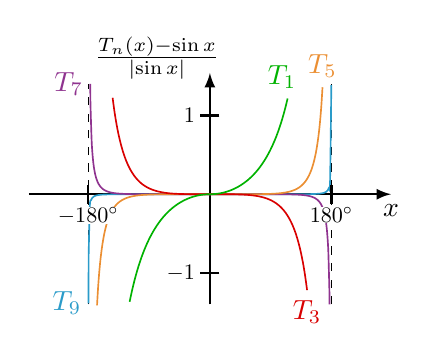
\begin{tikzpicture}
  \message{^^JSine difference}
  \def\A{1.0}    % amplitude
  \def\xmax{2.3} % max x axis
  \def\ymax{1.4} % max y axis
  \def\om{(0.7*2*pi/(0.94*\xmax))} % angular frequency in radians
  \def\T{(2*pi/\om))} % period
  \def\reldif#1{{\A*((#1-sin(\om*180/pi*\x))/abs(sin(\om*180/pi*\x)))}} % relative difference
  \draw[->,thick] (0,-\ymax) -- (0,1.1*\ymax) node[right=1,above left=-6] {$\frac{T_n(x)-\sin x}{\abs{\sin x}}$};
  \draw[->,thick] (-\xmax,0) -- (\xmax,0) node[below] {$x$};
  \draw[dashed,very thin] ({\T/2},-\ymax) -- ({\T/2},\ymax);
  \draw[dashed,very thin] ({-\T/2},-\ymax) -- ({-\T/2},\ymax);
  \draw[Tline,mycyan,samples=100+\N,smooth,variable=\x,domain={0.4992*\T}:{-0.4992*\T}]
    ({0.499*\T},0.99*\ymax) --
    plot(\x,\reldif{\om*\x-\om^3/6*(\x)^3+\om^5/120*(\x)^5-(\om/3.38*\x)^7+(\om/4.1472*\x)^9})
    -- ({-0.499*\T},-0.99*\ymax) node[left=-1] {$T_9$};
  \draw[Tline,mypurple,samples=100+\N,smooth,variable=\x,domain={0.492*\T}:{-0.492*\T}]
    ({0.492*\T},-\ymax) --
    plot(\x,\reldif{\om*\x-\om^3/6*(\x)^3+\om^5/120*(\x)^5-(\om/3.38*\x)^7})
    -- ({-0.492*\T},\ymax)
    node[left=-1] {$T_7$};
  \draw[Tline,myorange,samples=100+\N,smooth,variable=\x,domain={-0.464*\T}:{0.464*\T}]
    plot(\x,\reldif{\om*\x-\om^3/6*(\x)^3+\om^5/120*(\x)^5})
    node[above] {$T_5$};
  \draw[Tline,myred,samples=\N,smooth,variable=\x,domain={-0.40*\T}:{0.40*\T}]
    plot(\x,\reldif{\om*\x-\om^3/6*(\x)^3})
    node[below=0] {$T_3$};
  \draw[Tline,mygreen,samples=\N,smooth,variable=\x,domain={-0.33*\T}:{0.32*\T}]
    plot(\x,\reldif{\om*\x})
    node[left=2,above=0] {$T_1$};
  \tick{0,{\A}}{0} node[left=-1,scale=0.8] {$1$};
  \tick{0,{-\A}}{0} node[left=-1,scale=0.8] {$-1$};
  \tick{{\T/2},0}{90} node[below=1,scale=0.8,fill=white,inner sep=0] {\SI{180}{\degree}};
  \tick{{-\T/2},0}{90} node[below=1,scale=0.8,fill=white,inner sep=0] {\SI{-180}{\degree}};
\end{tikzpicture}


% COS - difference zoom
% (1-(10/180*pi)^2/2-cos(10/180*pi))/cos(10/180*pi) = -0.0039%
% (1-(15/180*pi)^2/2-cos(15/180*pi))/cos(15/180*pi) = -0.0202%
% (1-(20/180*pi)^2/2-cos(20/180*pi))/cos(20/180*pi) = -0.0656%
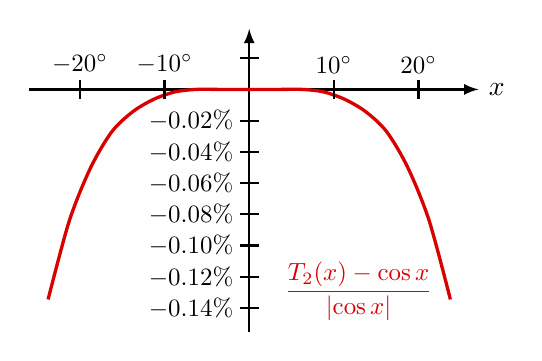
\begin{tikzpicture}
  \message{^^JCosine difference zoom}
  \def\A{2000}     % amplitude
  \def\xmax{2.8} % max x axis
  \def\ymax{2.2} % max y axis
  \def\om{(0.068*2*pi/(0.94*\xmax))} % angular frequency in radians
  \def\T{(2*pi/\om))} % period
  \def\reldif#1{{\A*((#1-cos(\om*180/pi*\x))/abs(cos(\om*180/pi*\x)))}} % relative difference
  \draw[->,thick] (0,-1.4*\ymax) -- (0,0.35*\ymax); %node[above=2,left=-6,scale=0.8] {$\dfrac{T_n-\sin}{\abs{\sin}}$}; % [\%]
  \draw[->,thick] (-\xmax,0) -- (1.04*\xmax,0) node[right] {$x$}; %\theta
  \draw[Tline,very thick,myred,samples=20,smooth,variable=\x] % improve rounding errors
    plot[domain={-0.066*\T}:{0.066*\T}](\x,{\A*(-(\om*\x/2.21336)^4+(\om*\x/2.9938)^6)/abs(1-(\om*\x)^2/2+(\om*\x/2.21336)^4-(\om*\x/2.9938)^6)})
    node[above=3,left=3,scale=0.9] {$\dfrac{T_2(x)-\cos x}{\abs{\cos x}}$}; %{$T_1$};
  \tick{0,{0.02/100*\A}}{0};
  \foreach \i in {0.02,0.04,0.06,0.08,0.10,0.12,0.14}{
    %\tick{0,{\i/100*\A}}{0} node[left=-1,scale=0.9] {$\i\%$};
    \tick{0,{-\i/100*\A}}{0} node[left=-1,scale=0.9] {$-\i\%$};
  }
  \foreach \x in {10,20}{
    \tick{{\x/360*\T},0}{-90} node[above=-1,scale=0.9] {\SI{\x}{\degree}};
    \tick{{-\x/360*\T},0}{-90} node[above=-1,scale=0.9] {\SI{-\x}{\degree}};
  }
\end{tikzpicture}


% SIN - difference zoom
% (10/180*pi-sin(10/180*pi))/sin(10/180*pi) = 0.51%
% (14/180*pi-sin(14/180*pi))/sin(14/180*pi) = 1.00%
% (15/180*pi-sin(15/180*pi))/sin(15/180*pi) = 1.15%
% (15/180*pi-sin(15/180*pi))/sin(15/180*pi) = 1.15%
% (20/180*pi-sin(20/180*pi))/sin(20/180*pi) = 2.06%
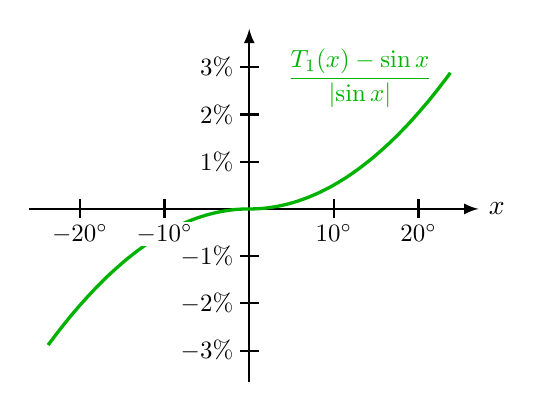
\begin{tikzpicture}
  \message{^^JSine difference zoom}
  \def\A{60}     % amplitude
  \def\xmax{2.8} % max x axis
  \def\ymax{2.2} % max y axis
  \def\om{(0.068*2*pi/(0.94*\xmax))} % angular frequency in radians
  \def\T{(2*pi/\om))} % period
  \def\reldif#1{{\A*((#1-sin(\om*180/pi*\x))/abs(sin(\om*180/pi*\x)))}} % relative difference
  \draw[->,thick] (0,-\ymax) -- (0,1.04*\ymax); %node[above=2,left=-6,scale=0.8] {$\dfrac{T_n-\sin}{\abs{\sin}}$}; % [\%]
  \draw[->,thick] (-\xmax,0) -- (1.04*\xmax,0) node[right] {$x$}; %\theta
  %\draw[Tline,mycyan,samples=24,smooth,variable=\x,domain={-0.06*\T}:{0.06*\T}]
  %  plot(\x,\reldif{\om*\x})
  %  node[left=2,above=0] {$T_1$};
  \draw[Tline,very thick,mygreen,samples=50,smooth,variable=\x] % improve rounding errors
    %plot[domain={-0.065*\T}:{-0.001*\T}](\x,{\A* ((\om*\x)^3/6-(\om*\x/2.60517)^5+(\om*\x/3.38)^7)/abs((\om*\x)-(\om*\x)^3/6+(\om*\x/2.60517)^5-(\om*\x/3.38)^7) }) --
    %plot[domain={0.005*\T}:{0.065*\T}](\x,{\A* ((\om*\x)^3/6-(\om*\x/2.60517)^5+(\om*\x/3.38)^7)/abs((\om*\x)-(\om*\x)^3/6+(\om*\x/2.60517)^5-(\om*\x/3.38)^7) })
    plot[domain={-0.066*\T}:{-0.001*\T}](\x,{-\A*((\om*\x)^2/6-(\om*\x/2.60517)^4+(\om*\x/3.38)^6)/abs(1-(\om*\x)^2/6+(\om*\x/2.60517)^4-(\om*\x/3.38)^6)}) --
    plot[domain={0.001*\T}:{0.066*\T}](\x,{\A*((\om*\x)^2/6-(\om*\x/2.60517)^4+(\om*\x/3.38)^6)/abs(1-(\om*\x)^2/6+(\om*\x/2.60517)^4-(\om*\x/3.38)^6)})
    node[below=2,left=3,scale=0.9] {$\dfrac{T_1(x)-\sin x}{\abs{\sin x}}$}; %{$T_1$};
  \foreach \i in {1,2,3}{
    \tick{0,{\i/100*\A}}{0} node[left=-1,scale=0.9] {$\i\%$};
    \tick{0,{-\i/100*\A}}{0} node[left=-1,scale=0.9] {$-\i\%$};
  }
  \foreach \x in {10,20}{
    \tick{{\x/360*\T},0}{90} node[below=1,scale=0.9,fill=white,inner sep=1] {\SI{\x}{\degree}};
    \tick{{-\x/360*\T},0}{90} node[below=1,scale=0.9,fill=white,inner sep=1] {\SI{-\x}{\degree}};
  }
\end{tikzpicture}



\end{document}
